% LaTeX Präsentationsvorlage (2013) der TU Graz, rev12, 2013/01/31
% !TeX encoding = UTF-8
\documentclass{beamer}
% \documentclass[aspectratio=169]{beamer}
% \usetheme{tugraz2013}
% \usetheme[notes]{tugraz2013}
\usepackage{../common/beamerthemetugraz2013}
\usepackage{color}
\usepackage{multicol}
\usepackage{bbding}
\usepackage{wasysym}
\usepackage{caption}
\usepackage{array}
\usepackage{siunitx}
% \usepackage{minted}

\usepackage{listings}
\usepackage{xcolor}

\definecolor{codegreen}{rgb}{0,0.6,0}
\definecolor{codegray}{rgb}{0.5,0.5,0.5}
\definecolor{codepurple}{rgb}{0.58,0,0.82}
\definecolor{backcolour}{rgb}{0.95,0.95,0.92}
\lstdefinestyle{mystyle}{
    backgroundcolor=\color{backcolour},   
    commentstyle=\color{codegreen},
    keywordstyle=\color{magenta},
    numberstyle=\tiny\color{codegray},
    stringstyle=\color{codepurple},
    basicstyle=\ttfamily\footnotesize,
    breakatwhitespace=false,         
    breaklines=true,                 
    captionpos=b,                    
    keepspaces=true,                 
    numbers=left,                    
    numbersep=5pt,                  
    showspaces=false,                
    showstringspaces=false,
    showtabs=false,                  
    tabsize=2
}

\lstset{style=mystyle}

\usepackage{picture}
\usepackage{rotating}
\definecolor{darkred}{rgb}{0.85,0.16,0.0}
\definecolor{darkgreen}{rgb}{0.16,0.70,0.27}

\usepackage{xcolor}


\newcommand{\hrefu}[2]{\underline{\href{#1}{#2}}}
\newcommand{\hyperlinku}[2]{\underline{\hyperlink{#1}{#2}}}
\newcommand{\smallurl}[1]{%
  \begin{flushleft}
    \tiny\url{#1}
  \end{flushleft}
}
\newcommand{\smalltext}[1]{%
  \begin{flushleft}
    \tiny{#1}
  \end{flushleft}
}
\newcommand{\red}[1]{{\color{red} #1}}
\newcommand{\blue}[1]{{\color{blue} #1}}
\newcommand{\darkgreen}[1]{\textcolor{darkgreen}{#1}}
\newcommand{\darkred}[1]{\textcolor{darkred}{#1}}

\newcommand*{\vpointer}{\vcenter{\hbox{\scalebox{1.5}{\large\pointer}}}}

\newcommand{\be}[1]{\begin{equation} \label{#1}}
\newcommand{\ee}{\end{equation}}
\newcommand{\bea}[1]{\begin{eqnarray} \label{#1}}
\newcommand{\eea}{\end{eqnarray}}
\newcommand{\bean}{\begin{eqnarray*}}
\newcommand{\eean}{\end{eqnarray*}}

\newcommand{\non}{\nonumber\\}
\newcommand{\eq}[1]{(\ref{#1})}
\newcommand{\difp}[2]{\frac{\partial #1}{\partial #2}}
\newcommand{\br}{{\bf r}}
\newcommand{\bR}{{\bf R}}
\newcommand{\bA}{{\bf A}}
\newcommand{\bB}{{\bf B}}
\newcommand{\bE}{{\bf E}}
\newcommand{\bm}{{\bf m}}
%\renewcommand{\bm}{{\bf m}}
\newcommand{\bn}{{\bf n}}
\newcommand{\bN}{{\bf N}}
\newcommand{\bp}{{\bf p}}
\newcommand{\bP}{{\bf P}}
\newcommand{\bF}{{\bf F}}
\newcommand{\by}{{\bf y}}
\newcommand{\bz}{{\bf z}}
\newcommand{\bZ}{{\bf Z}}
\newcommand{\bV}{{\bf V}}
\newcommand{\bv}{{\bf v}}
\newcommand{\bu}{{\bf u}}
\newcommand{\bx}{{\bf x}}
\newcommand{\bX}{{\bf X}}
\newcommand{\bW}{{\bf W}}
\newcommand{\bJ}{{\bf J}}
\newcommand{\bj}{{\bf j}}
\newcommand{\bk}{{\bf k}}
\newcommand{\bTheta}{{\bf \Theta}}
\newcommand{\btheta}{{\boldsymbol\theta}}
\newcommand{\bOmega}{{\bf \Omega}}
\newcommand{\bomega}{{\boldsymbol\omega}}
\newcommand{\brho}{{\boldsymbol\rho}}
\newcommand{\rd}{{\rm d}}
\newcommand{\rJ}{{\rm J}}
\newcommand{\ph}{{\varphi}}
\newcommand{\te}{\theta}
\newcommand{\tht}{\vartheta}
\newcommand{\vpar}{v_\parallel}
\newcommand{\vparkb}{v_{\parallel k b}}
\newcommand{\vparkm}{v_{\parallel k m}}
\newcommand{\Jpar}{J_\parallel}
\newcommand{\ppar}{p_\parallel}
\newcommand{\Bpstar}{B_\parallel^*}
\newcommand{\intpi}{\int\limits_{0}^{2\pi}}
\newcommand{\summ}{\sum \limits_{m=-\infty}^\infty}
\newcommand{\tb}{\tau_b(\uv)}
\newcommand{\bh}{{\bf h}}
\newcommand{\cE}{{\cal E}}
\newcommand{\bsigma}{{\boldsymbol\sigma}}
\newcommand{\bS}{{\mathbf S}}
\newcommand{\bI}{{\mathbf I}}
\newcommand{\odtwo}[2]{\frac{\rd #1}{\rd #2}}
\newcommand{\pdone}[1]{\frac{\partial}{\partial #1}}
\newcommand{\pdtwo}[2]{\frac{\partial #1}{\partial #2}}
\newcommand{\ds}{\displaystyle} % commands


%% Titelblatt-Einstellungen
\title[]
{Python 11}
\author[E.~Wachmann]{\scriptsize Elias Wachmann
}
\date{2024} % \today für heutiges Datum verwenden
\institute[Institute of Theoretical and Computational Physics]
{
}
\instituteurl{www.tugraz.at}
% \institutelogo{kurz.pdf}
%~ \additionallogo{merged_logos}
\AtBeginSection[]{
  \begin{frame}
  \vfill
  \centering
  \begin{beamercolorbox}[sep=8pt,center,shadow=true,rounded=true]{title}
    \usebeamerfont{title}\insertsectionhead\par%
  \end{beamercolorbox}
  \vfill
  \end{frame}
}
\lstset{
    literate={Ö}{{\"O}}1
             {Ä}{{\"A}}1
             {Ü}{{\"U}}1
             {ß}{{\ss}}1
             {ü}{{\"u}}1
             {ä}{{\"a}}1
             {ö}{{\"o}}1
}

%%%%%%%%%%%%%%%%%%%%%%%%%%%%%%%%%%%%%%%%%%%%%%%%%%%%%%%%%%%%%%%%%%%%%%%%%%%%
\begin{document}
%%%%%%%%%%%%%%%%%%%%%%%%%%%%%%%%%%%%%%%%%%%%%%%%%%%%%%%%%%%%%%%%%%%%%%%%%%%%
\titleframe

%\begin{frame}
%  \frametitle{Outline}
%  \tableofcontents%[hideallsubsections] 
%  \note{
%  	Meine Präsentation ist wie folgt strukturiert \ldots
%  }
%\end{frame}

\section*{Content}

\begin{frame}
\frametitle{Content}
  \tableofcontents
\end{frame}

%%%%%%%%%%%%%%%%%%%%%%%%%%%%%%%%%%%%%%%%%%%%%%%%%%%%%%%%%%%%%%%%%%%%%%%%%%%%
\section{Uncertainties in Python}
\begin{frame}
  \frametitle{Uncertainties Package}
  The \texttt{uncertainties} package allows you to perform calculations with \hrefu{https://pythonhosted.org/uncertainties/}{\texttt{uncertainties}}
  It supports calculations with numbers that have uncertainties and automatically propagates those uncertainties through mathematical operations.\\
  \vspace{0.5cm}
  Install the package with \texttt{pip}:
  \begin{align*}
    \texttt{pip install uncertainties}
  \end{align*}
\end{frame}


\begin{frame}
  \frametitle{Basic Usage}
  To use the \texttt{uncertainties} package, you need to import the \texttt{ufloat} function, which creates numbers with uncertainties:
  \lstinputlisting[language=python, lastline=4]{examples/uncertainty1.py}
\end{frame}

\begin{frame}
  \frametitle{Propagation of Uncertainties}
  When you perform operations with these numbers, the uncertainties are automatically propagated using \hrefu{https://en.wikipedia.org/wiki/Propagation_of_uncertainty}{linear error propagation}\\
  \vspace{0.5cm}
  This is great, because you don't have to manually calculate the uncertainties of the results anymore. Just use the \texttt{nominal\_value} and \texttt{std\_dev} functions to get the result and its uncertainty:
\end{frame}

\begin{frame}
  \frametitle{Propagation of Uncertainties}
  \lstinputlisting[language=python, firstline=5, lastline=11]{examples/uncertainty1.py}
\end{frame}

\begin{frame}
  \frametitle{Mathematical Functions}
  The \texttt{uncertainties} package supports many mathematical functions, including trigonometric, exponential, and logarithmic functions:
  \lstinputlisting[language=python]{examples/uncertainty2.py}
\end{frame}


\begin{frame}
  \frametitle{Plotting with Uncertainties}
  You can also plot data with uncertainties using the \texttt{matplotlib} library:
  \lstinputlisting[language=python]{examples/uncertainty3.py}
\end{frame}

\begin{frame}
  \frametitle{Plotting with Uncertainties}
  \vspace{-5mm}
  \begin{figure}
    \centering
    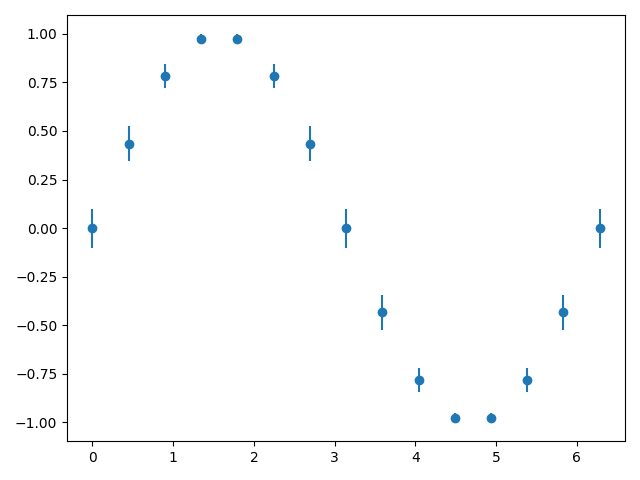
\includegraphics[width=0.75\textwidth]{examples/fig/plot.png}
  \end{figure}
\end{frame}

\begin{frame}
  \frametitle{Example: Beer-Lambert Law}
  The Beer-Lambert law relates the absorption of light to the properties of the material it passes through. It is given by:
  \begin{align*}
    I(x) = I_0 e^{-\alpha x}
  \end{align*}
  where $I(x)$ is the intensity of the light after passing through a material of thickness $x$, $I_0$ is the initial intensity, and $\alpha$ is the absorption coefficient.\\
\end{frame}

\begin{frame}
  \frametitle{Example: Beer-Lambert Law}
  Suppose we have the following measurements:
  % table with 5 measurements for different x: 
  \begin{table}[H]
    \centering
    \begin{tabular}{|c|c|c|}
      \hline
      $x$ & $I(x)$ & $\Delta I(x)$ \\
      \hline
      0.0 & 1.0 & 0.1 \\
      0.5 & 0.6 & 0.1 \\
      1.0 & 0.4 & 0.1 \\
      1.5 & 0.3 & 0.1 \\
      2.0 & 0.2 & 0.1 \\
      \hline
  \end{tabular}
  \end{table}
  and we want to determine the absorption coefficient $\alpha$ using a fit to the Beer-Lambert law.
\end{frame}
\begin{frame}
  \frametitle{Example: Beer-Lambert Law}
  \vspace{-5mm}
  \begin{figure}
    \centering
    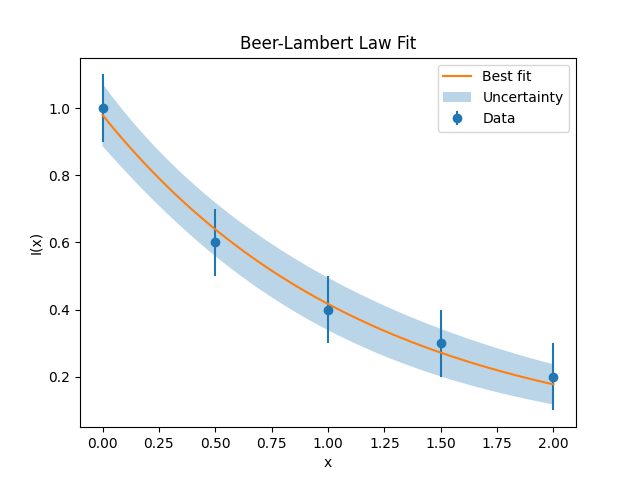
\includegraphics[width=0.75\textwidth]{examples/fig/beerLambert.png}
  \end{figure}
\end{frame}
\section{Test Driven Development (TDD) in Python}
\begin{frame}
  \frametitle{Introduction to TDD}
  Test Driven Development (TDD) is a software development methodology in which tests are written before the code that needs to be tested.
  \begin{itemize}
    \item Write a test for the new functionality.
    \item Write the minimum amount of code to make the test pass.
    \item Refactor the code while ensuring that all tests still pass.
  \end{itemize}
\end{frame}

\begin{frame}
  \frametitle{Benefits of TDD}
  \begin{itemize}
    \item Ensures code quality and correctness.
    \item Facilitates better design and architecture.
    \item Provides documentation for the code.
    \item Helps in detecting bugs early.
  \end{itemize}
\end{frame}

\begin{frame}
  \frametitle{TDD Cycle}
  The TDD cycle consists of the following steps:
  \begin{enumerate}
    \item \textbf{Red:} Write a test that fails.
    \item \textbf{Green:} Write the minimal code to pass the test.
    \item \textbf{Refactor:} Improve the code while ensuring tests pass.
  \end{enumerate}
\end{frame}

\begin{frame}
  \frametitle{Example: Simple Calculator}
  Let's consider a simple calculator as an example. We want to implement an \texttt{add} function.
  \lstinputlisting[language=python, lastline=2]{examples/calculator.py}
  \vspace{5mm}
  Let us write a test for this function \dots
\end{frame}

\begin{frame}
  \frametitle{Writing Tests with Pytest}
  Pytest is a testing framework for Python that makes it easy to write simple and scalable test cases.
  Install pytest using pip:
  \begin{align*}
  \texttt{pip install pytest}
  \end{align*}
  We specify the test functions using the \texttt{test\_} prefix. They are automatically detected and run by Pytest.
\end{frame}

\begin{frame}
  \frametitle{Pytest Example}
  Here is an example of a test for the \texttt{add} function using Pytest:
  \lstinputlisting[language=python]{examples/test\_calculator.py}
  Place this test in a file prefixed with \texttt{test\_} (e.g., \texttt{test\_calculator.py}) into the same directory as the code.
\end{frame}

\begin{frame}
  \frametitle{Running Tests}
  To run the tests, simply execute the following command in the terminal:
  \begin{align*}
  \texttt{pytest}
  \end{align*}
  Pytest will automatically discover and run all the test files that match the pattern \texttt{test\_*.py}.
\end{frame}

\begin{frame}
  \frametitle{Refactoring}
  After making the test pass, you can refactor the code to improve its quality. Ensure that all tests still pass after refactoring.
  \lstinputlisting[language=python]{examples/calculator\_refactored.py}
\end{frame}
\begin{frame}
  \frametitle{Refactoring}
  \lstinputlisting[language=python]{examples/test\_calculator\_refactored.py}
\end{frame}
\begin{frame}
  \frametitle{Best Practices}
  \begin{itemize}
    \item Write small, focused tests.
    \item Use descriptive test names.
    \item Keep tests independent.
    \item Regularly run all tests.
    \item Refactor tests along with the code.
  \end{itemize}
\end{frame}

\begin{frame}
  \frametitle{Conclusion}
  Test Driven Development (TDD) helps in ensuring \textbf{code quality}, \underline{detecting bugs early}, and improving the design and architecture of the code.\\
  Pytest is a powerful and easy-to-use testing framework for implementing TDD in Python.\\
  Start with small steps, and iteratively build a robust suite of tests alongside your code.
\end{frame}

\section{What is object oriented programming?}
\begin{frame}
  \frametitle{Intro to object oriented programming}
  How do we classify things in the real world?\\
  \vspace{5mm}
  We group them by their properties and their behavior.\\
  \vspace{5mm}
  An \textbf{object} like a planet can be described by its properties like mass, radius, position, velocity, etc.\\
  \vspace{5mm}
  We can also describe its behavior, like how it moves around the sun.\\
\end{frame}
\begin{frame}
  \frametitle{What are classes?}
  \textbf{Classes} are a way to abstract real world things into categories.\\
  \begin{minipage}[t]{0.55\textwidth}
    \vspace{-3cm}
    Not all planets are the same, but they can be described by the same properties and behavior.\\
    We can use a \textbf{class} that describes the properties and behavior of a planet (an \textbf{object}).\\
  \end{minipage}%
  \hspace{5mm}
  \begin{minipage}[t]{0.35\textwidth}
    \centering
    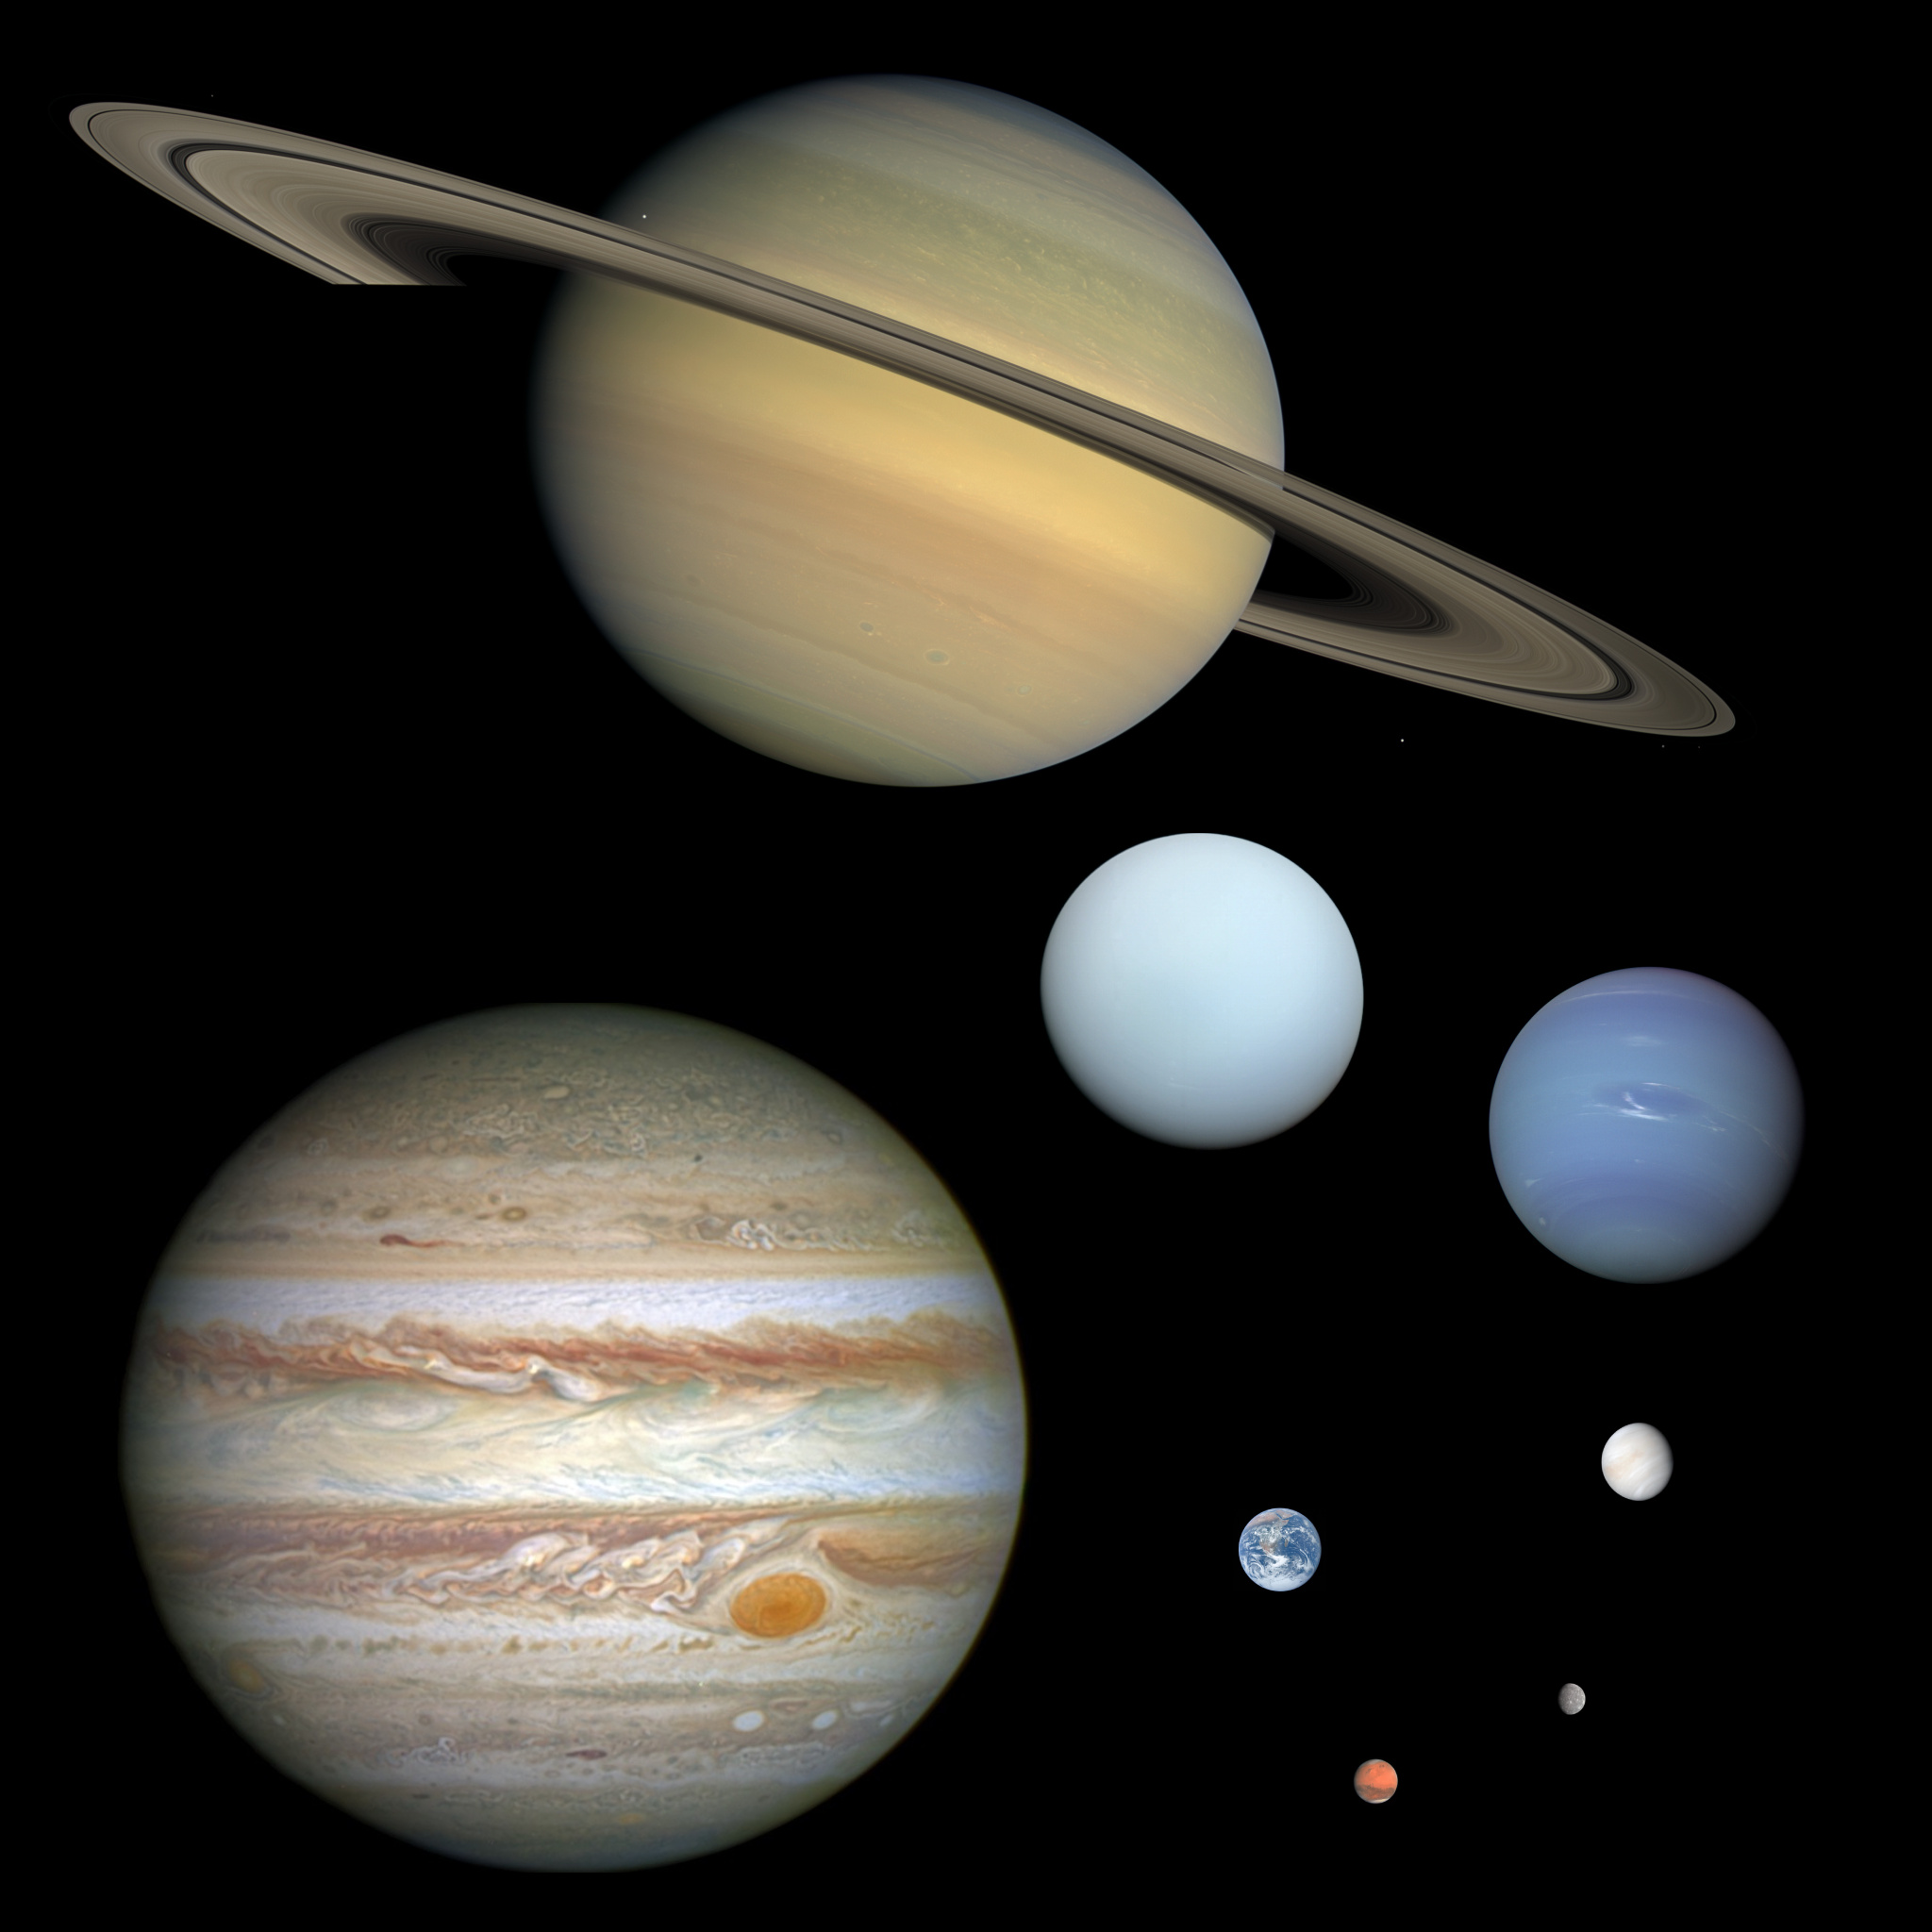
\includegraphics[width=0.9\textwidth]{examples/fig/Planet_collage_to_scale.jpg}
    \smallurl{https://upload.wikimedia.org/wikipedia/commons/c/cf/Planet_collage_to_scale.jpg}
\end{minipage}
\end{frame} 
\begin{frame}
  \frametitle{Describe objects within a class}
  How can we distinguish between different planets now?\\
  \vspace{5mm}
  \textbf{Earth}: m = \SI{5.97e24}{kg}, r = 6371 km, \dots\\
  \vspace{5mm}
  \textbf{Mars}: m = \SI{6.41e23}{kg}, r = 3389.5 km, \dots\\
  \vspace{5mm}
  \textbf{Jupiter}: m = \SI{1.90e27}{kg}, r = 69911 km, \dots\\
\end{frame}
\section{Python classes}
\begin{frame}
  \frametitle{Let's define a Planet class}
  In python we can define a class like this:\\
  \lstinputlisting[language=python, lastline=5]{examples/planets.py}
  \vspace{5mm}
  The \textbf{\hrefu{https://docs.python.org/3/tutorial/classes.html}{class}}-keyword tells python that we want to define a class.\\
\end{frame}
\begin{frame}
  \frametitle{What is the \_\_init\_\_ function?}
  The \textbf{\hrefu{https://docs.python.org/3/reference/datamodel.html\#object.__init__}{\_\_init\_\_}} function is called when we create a new object of the class.\\
  \vspace{5mm}
  Objects are therefore concrete \textbf{instances} of a class.\\
  \vspace{5mm}
  In our example the Planet class takes the arguments \textbf{mass} and \textbf{radius} and stores them as \textbf{attributes} of the object.\\
  \vspace{5mm}
  How can we access these attributes and what is the \textbf{\hrefu{https://docs.python.org/3/faq/programming.html\#what-is-self}{self}}-keyword?\\
\end{frame}
\begin{frame}
  \frametitle{Idea behing self keyword}
  The \textbf{self} keyword is a reference to the object itself.\\
  \vspace{5mm}
  What does this mean?\\
  \vspace{5mm}
  2 options: 
  \begin{itemize}
    \item Just accept it as is and use it.\\
    \item Understand what it does.\\
  \end{itemize}
  When we create an object of a class, we can access its attributes and methods using the \textbf{self} keyword inside the class.\\
\end{frame}
\begin{frame}
  \frametitle{Pythons self keyword}
  The \textbf{self} keyword is a reference to the object itself.\\
  \lstinputlisting[language=python,firstline=2, lastline=5]{examples/planets.py}
  This means: If you want to create an attribute of a class, you simply write \texttt{\textbf{self}.variable\_name}\\
  \vspace{5mm}
  \textbf{self} also has to be passed in as the first argument to every function defined inside the class (for context)! 
\end{frame}
\begin{frame}
  \frametitle{Methods -- class functions}
  \textbf{\hrefu{https://docs.python.org/3/tutorial/classes.html\#methods}{Methods}} are functions inside a class. They can only be accessed by objects of that class and \textbf{self} is their first argument.  
  \lstinputlisting[language=python, lastline=8]{examples/planets.py}
\end{frame}
\begin{frame}
  \frametitle{Let's create a Planet}
  Finally let's create a planet object: 
  \lstinputlisting[language=python, firstline=13, lastline=14]{examples/planets.py}
  Just pass in the initial arguments just like you would for functions. 
  \lstinputlisting[language=python, firstline=15, lastline=16]{examples/planets.py}
  We can now call our defined class method on objects. 
\end{frame}
\begin{frame}
  \frametitle{Modify objects}
  Certainly a method can modify attributes of an object like in the following example the name. 
  \lstinputlisting[language=python, firstline=10, lastline=12]{examples/planets.py}  

  \lstinputlisting[language=python, firstline=17]{examples/planets.py}  
  This only changes the name of the \glq earth\grq-object while the \glq mars\grq-object is not affected. 
\end{frame}
%%%%%%%%%%%%%%%%%%%%%%%%%%%%%%%%%%%%%%%%%%%%%%%%%%%%%%%%%%%%%%%%%%%%%%%%%%%%
% \section{Dunder-methods}
% \begin{frame}
%   \frametitle{Dunder-methods}
%   \textbf{\hrefu{https://docs.python.org/3/reference/datamodel.html\#special-method-names}{Dunder-methods}} are special methods that are called by python in certain situations.\\
%   \vspace{5mm}
%   We have seen the \textbf{\hrefu{https://docs.python.org/3/reference/datamodel.html\#object.__init__}{\_\_init\_\_}} method, which is called when a new object is created, before.\\
%   Further examples include: 
%   \begin{itemize}
%     \item \textbf{\hrefu{https://docs.python.org/3/reference/datamodel.html}{\_\_str\_\_}} method is called when we try to convert an object to a string.\\
%     \item \textbf{\hrefu{https://docs.python.org/3/reference/datamodel.html}{\_\_add\_\_}} method is called for + operator.\\
%     \item  \textbf{\hrefu{https://docs.python.org/3/reference/datamodel.html}{\_\_lt\_\_, \_\_le\_\_, \_\_eq\_\_, \_\_ne\_\_, \_\_gt\_\_, \_\_ge\_\_}} methods used for comparisons. 
%   \end{itemize}
% \end{frame}
% \begin{frame}
%   \frametitle{Dunder-methods -- Examples}
%   One can now implement dunder methods for our custom classes to make certain functionality (like comparisons between objects) possible.\\
%   \lstinputlisting[language=python, firstline=13, lastline=19]{examples/planets\_dunder.py}
% \end{frame}
% \begin{frame}
%   \frametitle{Dunder-methods -- Iterators}
%   \textbf{\hrefu{https://docs.python.org/3/reference/datamodel.html\#object.__iter__}{\_\_iter\_\_}} and \textbf{\hrefu{https://docs.python.org/3/reference/datamodel.html\#object.__next__}{\_\_next\_\_}} are special methods that allow us to iterate over objects.\\
%   \vspace{5mm}
%   While \textbf{\_\_iter\_\_} returns an iterator object, \textbf{\_\_next\_\_} returns the next element of the iterator.\\
%   \vspace{5mm}
%   This allows us to specify what a while/for loop should do when it encounters an object of our class.\\
% \end{frame}
% \begin{frame}
%   \frametitle{Dunder-methods -- Iterators -- Example}
%   Let's define a new class: 
%   \lstinputlisting[language=python, lastline=8]{examples/iter.py}
%   \dots
% \end{frame}
% \begin{frame}
%   \frametitle{Dunder-methods -- Iterators -- Example}
%   \vspace{-10mm}
%   \lstinputlisting[language=python, firstline=11, lastline=22]{examples/iter.py}
%   \dots
% \end{frame}
% \begin{frame}
%   \frametitle{Dunder-methods -- Iterators -- Example}
%   \vspace{-10mm}
%   \lstinputlisting[language=python, firstline=24]{examples/iter.py}
% \end{frame}
% %%%%%%%%%%%%%%%%%%%%%%%%%%%%%%%%%%%%%%%%%%%%%%%%%%%%%%%%%%%%%%%%%%%%%%%%%%%%
% \section{Inheritance}

\end{document}
%%%%%%%%%%%%%%%%%%%%%%%%%%%%%%%%%%%%%%%%%%%%%%%%%%%%%%%%%%%%%%%%%%%%%%%%%%%%

%% EOF
